\lhead[]{}
\rhead[]{}
\renewcommand{\headrulewidth}{0pt}
\chapter*{about this book} 
This is a book about a toy. A toy that was the first of its kind. A kind of toy that has never really caught on,
though maybe its moment lies some way in the future. 

A static picture does the toy no justice, but we will show a few anyway. If you do not know what \textit{Psychedelia} is, they
might at least give you a flavour of this game that is not a game. 
\begin{figure}[H]
    \begin{adjustbox}{width=10cm,center}
    \frame{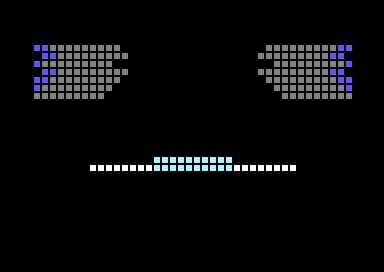
\includegraphics{src/preface/p1.png}}%
      \hspace{0.1cm}
    \frame{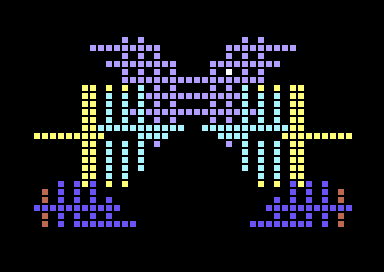
\includegraphics{src/preface/p2.png}}%
    \end{adjustbox}
\end{figure}
\vspace{-0.8cm}
\begin{figure}[H]
    \begin{adjustbox}{width=10cm,center}
    \frame{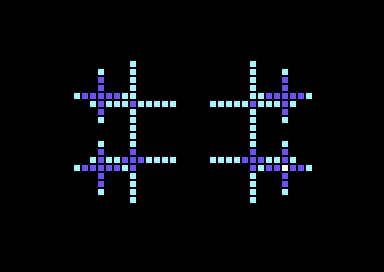
\includegraphics{src/preface/p3.png}}%
      \hspace{0.1cm}
    \frame{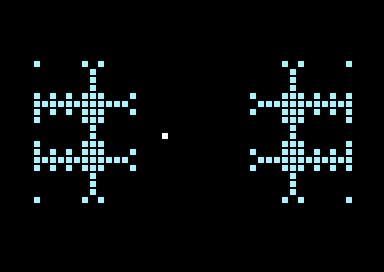
\includegraphics{src/preface/p4.png}}%
    \end{adjustbox}
\end{figure}

\textit{Psychedelia} is a kind of interactive pixel painter and was the first of its kind. 
The best description of what this toy is about is in the words of its creator, Jeff Minter, who at the time was
a 25 year old programmer of eccentric video games for the Commodore 64:

\begin{figure}[H]
    \centering
    \begin{adjustbox}{width=12cm,center}
    \frame{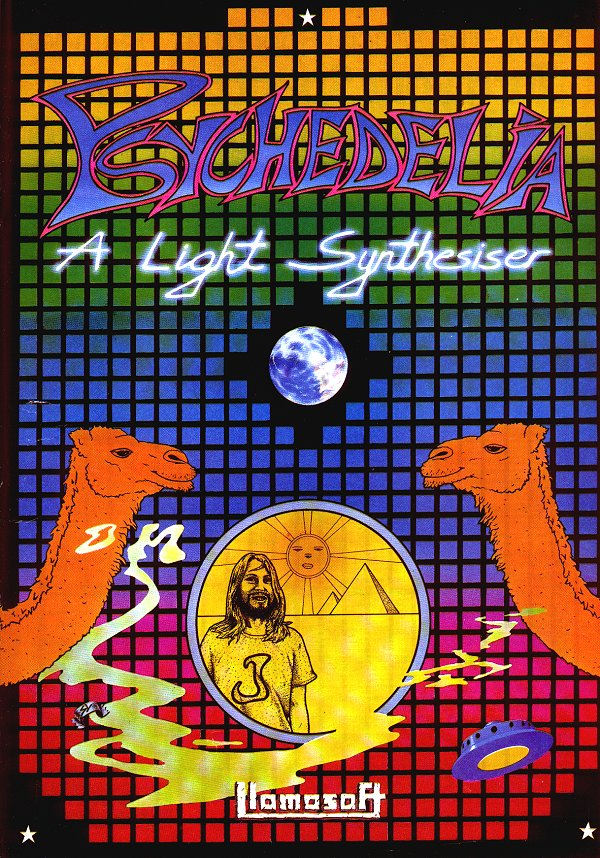
\includegraphics{src/preface/psychedelia.jpg}}%
    \end{adjustbox}
  \caption{Cover art by Steinar Lund for the commercial edition of \textit{Psychedelia}}
\end{figure}

\begin{definition}[Jeffrey Says]
\setlength{\intextsep}{0pt}%
\setlength{\columnsep}{3pt}%
\begin{wrapfigure}{l}{0.12\textwidth}

\includegraphics[width=\linewidth]{src/callout/psych.png} 
\end{wrapfigure}
\small
It just felt wonderfully new, and somehow primal... it was like the patterns
  and mandalas that have fascinated humans for millennia, but come to life,
  under your control... in fact I was so moved by what I'd found that at first
  I refused to make it commercial... I felt that something so basic and lovely
  deserved more than just being another thing to be sold and profited from. I
  actually gave that first algorithm away in listing form to a computer
  magazine. But my parents argued successfully that there was no shame in
  making some money from it, and so in due course I created a somewhat expanded
  version with more patterns and control options, and that is what was released
  as \textit{Psychedelia}.

  I called the program a "light synthesiser", and advertised it as a new,
  non-competitive form of entertainment... no enemies, no killing, just light
  and colour. 
\end{definition}

This book is not about the history of this game. This book is an exploration of the computer code that makes
the game tick. We discuss the algorithm used to generate all these pretty pictures in detail and dissect the
pictures themselves. We pick over the code in sometimes minute detail to try to figure out its workings.

We are going to take apart the toy to see how it works. The pieces are all over the floor and they seem to be made
of strange-looking computer instructions, I hope we know what we're doing...


\section*{note on the text}
The version you are reading is still a few revisions away from a
finished product. If you find the writing hard going or the attempts to explain things difficult
to follow, by all means \href{https://github.com/mwenge/psypixels/issues}{\textcolor{blue}{leave me a note}} and
I will gratefully accept your complaint. In the meantime, please skip over any blemishes
to the next pretty picture or promising-looking block of text.

The full source code is available in \href{https://github.com/mwenge/psychedelia}{\textcolor{blue}{its own Github repository}}. 
You should find that it matches exactly the snippets of code provided in the book, though in some cases the extracts in the book have been edited
and reformatted for brevity.


Rob Hogan (\href{https://mastodon.social/@mwenge}{\textcolor{blue}{@mwenge}})\\
Dublin \the\year{} \\

\clearpage
\blankpage
\vspace*{\fill}
\begin{figure}[H]
    \centering
      
\includegraphics[width=8cm]{src/cover/title_page.png}%
\end{figure}
\vspace*{\fill}
\thispagestyle{empty}%
\clearpage
\blankpage

